% !TEX root = ../master-thesis.tex


\begin{figure}
    \centering
    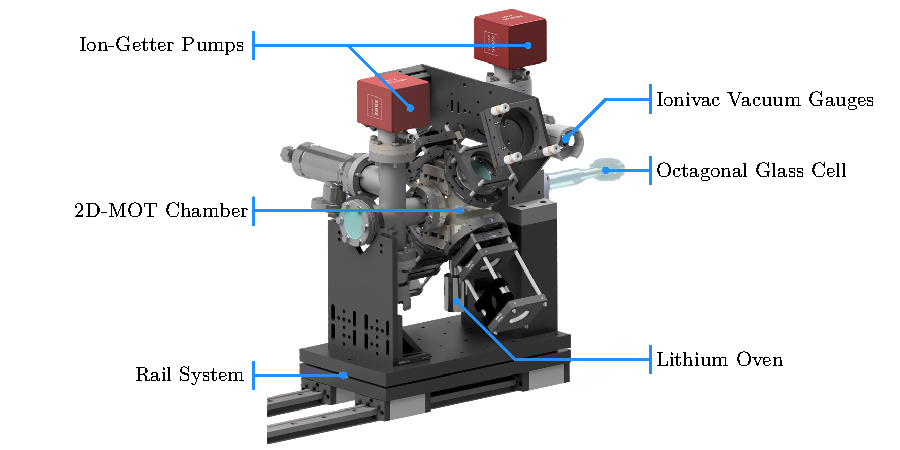
\includegraphics{fig-ai/setup.pdf} 
    \caption{
    \textbf{Rendering of the vacuum chamber setup.} 
    $^6$Li vapor emitted from the oven is captured and cooled by a 2D-MOT. A push beam transfers the pre-cooled atoms into the octagonal glass cell, where a 3D-MOT further cools and confines the atoms in all spatial directions, preparing them for subsequent loading into an ODT.
    }
    \label{fig:setup}
\end{figure}



The experimental apparatus is designed to realize and investigate complex quantum many-body dynamics using ultracold fermionic $^6$Li atoms. The primary objective of the setup is to create highly controllable initial quantum states, facilitate quantum simulation of the Fermi-Hubbard model, and enable precise measurements of quantum observables, such as entanglement entropy and particle correlations.

The experimental procedure starts with $^6$Li atoms emitted from an atomic oven. Lithium atoms are first collected and precooled in a two-dimensional magneto-optical trap (2D MOT), effectively capturing a high flux of atoms. From there, the atoms are transferred into a three-dimensional magneto-optical trap (3D MOT) for additional cooling and confinement, reaching temperatures near the Doppler limit (approximately 141~$\mu$K for $^6$Li) \cite{culemann_construction_2024, huang_construction_2024}.

Following the 3D MOT, atoms are loaded into a crossed optical dipole trap (ODT), generated by intersecting laser beams, creating a stable potential. At this stage, evaporative cooling further reduces the temperature significantly below quantum degeneracy conditions, reaching regimes where a molecular Bose-Einstein condensate (mBEC) can form. One of the first tasks within this thesis involved developing software for analyzing mBEC preparation data. Figure~\ref{fig:mbec} illustrates results from this analysis, demonstrating the phase space density (PSD) increasing with reduced temperature due to evaporative cooling (Fig.~\ref{fig:mbec}a). Measured atom density profiles at various temperatures show a characteristic bimodal distribution at low temperatures, indicative of mBEC formation (Fig.~\ref{fig:mbec}b). Fitting a Gaussian profile to the thermal wings of this distribution (red points in Fig.~\ref{fig:mbec}c) clearly reveals a central peak representing the condensed fraction (blue shaded area in Fig.~\ref{fig:mbec}c). While the generation of a molecular BEC is not part of the envisioned quantum simulation sequence, it impressively demonstrates the capabilities of the cooling and trapping system to reach quantum degeneracy.

\begin{figure}
    \centering
    \addletter{130}{a}
    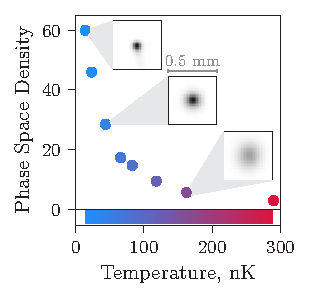
\includegraphics{fig-ai/m-bec-1-joined.pdf}
    \addletter{130}{b}
    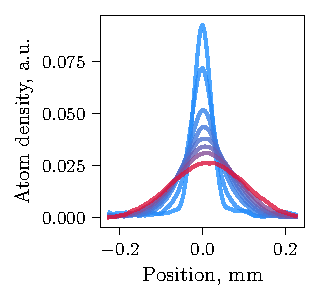
\includegraphics{fig-py/m-bec-2.pdf}
    \addletter{130}{c}
    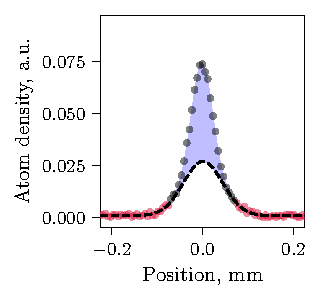
\includegraphics{fig-py/m-bec-3.pdf}
    \caption{
        \textbf{Molecular Bose-Einstein condensate data.}
        (a) Phase space density (PSD) increases as temperature decreases via evaporative cooling, indicating condensation onset. 
        (b) Measured atom density profiles normalized to unit area; color encodes temperature as in (a).
        (c) At low temperature, the profile shows a bimodal shape: a Gaussian fit to thermal wings (red dots) underestimates the central peak, revealing the mBEC component (blue area).
    }
    \label{fig:mbec}
\end{figure}



After reaching degeneracy in the ODT, atoms are adiabatically transferred into an optical tweezer array, implemented using crossed acousto-optic deflectors (AODs). These tweezers provide deterministic preparation of quantum states with single-site control, enabling initialization of specific many-body configurations essential for studying Fermi-Hubbard physics beyond thermal equilibrium. Precise atom number management is achieved through the spilling technique, which utilizes a magnetic field gradient and controlled reduction of tweezer depth to selectively retain atoms in low vibrational states \cite{culemann_construction_2024, huang_construction_2024}.

A critical aspect of our experiment is precise atom counting, particularly important when recapturing atoms from tweezers back into the MOT for calibration purposes. Atom number quantization can be clearly observed through fluorescence signal histograms, obtained with prolonged exposure times in a MOT loaded with a small number of atoms. Figure~\ref{fig:spillingadd}a shows discrete peaks corresponding to integer atom numbers, confirming accurate and reliable single-atom counting.

Future experimental plans involve transferring precisely prepared atoms into optical lattices engineered to simulate the Fermi-Hubbard model. The implemented lattice system features tunable geometry, capable of switching between square and triangular configurations without hardware modifications \cite{dux_optical_2023}. This flexibility enables systematic investigation of geometry-dependent phenomena in strongly correlated fermions. For vertical confinement, an accordion z-lattice provides the necessary two-dimensional character essential for Fermi-Hubbard physics while maintaining single-site resolution during imaging (detailed implementation described in \cite{huang_construction_2024}). Lattice depth and geometry, as well as disorder potentials, can be precisely tuned. Disorder is introduced using a digital micromirror device (DMD), enabling controlled studies of localization phenomena. 

To achieve single-site resolution with lattice spacings below the free-space imaging limit, a matter-wave magnifier (MWM) system is being implemented. Two additional harmonic trapping potentials have been installed for this purpose. The MWM coherently expands atomic distributions before imaging, enabling site-resolved detection in lattices with sub-micrometer spacing. Detailed theoretical and numerical analysis of the MWM system is presented in Section~\ref{sec:mwm}.

High-resolution, spin-resolved imaging is crucial for detailed characterization of quantum states in Fermi-Hubbard systems. The imaging system employs fluorescence-based free-space techniques, enabling rapid and high-fidelity spin detection with single-shot capability. Atoms are transferred to stretched hyperfine states, optimizing photon collection efficiency through closed cycling transitions. The implementation of spin-resolved detection represents a key development in this work. As part of this thesis, a complete distribution board for imaging and radiofrequency beam control was designed and assembled, including combining optics, acousto-optic modulator stages, and fiber coupling systems (detailed in Section~\ref{subsec:imaging-setup}). This enables simultaneous detection of both hyperfine ground states in a single experimental shot, providing direct access to local magnetization and spin correlations essential for characterizing magnetic phases in the Fermi-Hubbard model.

Control over atomic spin states is executed using dedicated radiofrequency (RF) and microwave (MW) antennas. The PCB-based RF antenna drives MHz-range spin transitions, while the MW loop antenna efficiently couples to hyperfine transitions, enabling coherent manipulation critical for state preparation, spin-selective procedures, and precise quantum control. These capabilities are essential for implementing spin-selective spilling protocols and preparing arbitrary spin-resolved configurations.

The entire experimental cycle (including state preparation, evolution, and measurement) is optimized for rapid repetition with a cycle time of approximately 2 seconds, allowing statistically robust data collection. The integration of all subsystems (from atomic source through deterministic state preparation to spin-resolved detection) provides a complete platform for investigating quantum many-body dynamics in engineered Fermi-Hubbard systems. The combination of programmable initial states, tunable Hamiltonians, and high-fidelity measurements enables systematic exploration of phenomena ranging from equilibrium quantum phases to out-of-equilibrium dynamics including thermalization and localization.


